\chapterimage{MathCover.png} % Chapter heading image

\chapter{Math Problems - Part I}

\section{Unit Conversions}\index{Unit Conversions}
\subsection{Example Problems} \index{Example Problems}  
\begin{enumerate}
\item Convert 1000 $ft^3$ to cu. yards:\\
$1000 \cancel{ft^3}*\dfrac{cu.yards}{27\cancel{ft^3}} = 37 cu.yards$\\

\item Convert 3.5 $ft^3/sec$ to MGD:\\
$\dfrac{3.5 \enspace \cancel{ft^3}}{\cancel{sec}} * \dfrac{7.48\cancel {\enspace gal}}{\cancel{ft^3}} * \dfrac{MG}{\enspace 10^6 \cancel{gal}}* \dfrac{1440*60 \enspace \cancel{sec}}{day}=  2.3 \enspace MGD$\\

\item Convert 1,000 L water to lbs:\\
$1000 \enspace \cancel{L}*\dfrac {\cancel{gal}}{3.785 \enspace \cancel{L}}*\dfrac{8.34 \enspace lbs}{\cancel{gal}}\enspace  = 2,203 \enspace lbs$\\
$(Note:8.34 \enspace lbs/gal \enspace is \enspace density \enspace of \enspace water - a \enspace constant)$\\ 
\end{enumerate}


\subsection{Practice Problems} \index{Practice Problems}
\begin{enumerate}
\item Given 1 ft = 30.48 cm and 5,280 ft = mile, convert 3 miles to cm\\


\item The wastewater flow to a treatment plant has a velocity of 61 cm/s. What is this velocity expressed in ft/min. Given: 1 ft = 30.48 cm\\

\item As an operator of a wastewater plant you are treating a flow of 21 MGD, what is the flow in gallons per minute?\\
\end{enumerate}

\newpage

\section{Area \& Volume}\index{Area \& Volume}
 
\subsection{Example Problems} \index{Example Problems} 
\begin{enumerate}
\item The floor of a rectangular building is 20 feet long by 12 feet wide and the inside walls are 10 feet high. Find the total surface area of the inside walls of this building\\
Solution:\\
\begin{center}
\begin{tikzpicture}
	%%% Edit the following coordinate to change the shape of your
	%%% cuboid
      
	%% Vanishing points for perspective handling
	\coordinate (P1) at (-7cm,1.5cm); % left vanishing point (To pick)
	\coordinate (P2) at (8cm,1.5cm); % right vanishing point (To pick)

	%% (A1) and (A2) defines the 2 central points of the cuboid
	\coordinate (A1) at (0em,0cm); % central top point (To pick)
	\coordinate (A2) at (0em,-2cm); % central bottom point (To pick)

	%% (A3) to (A8) are computed given a unique parameter (or 2) .8
	% You can vary .8 from 0 to 1 to change perspective on left side
	\coordinate (A3) at ($(P1)!.8!(A2)$); % To pick for perspective 
	\coordinate (A4) at ($(P1)!.8!(A1)$);

	% You can vary .8 from 0 to 1 to change perspective on right side
	\coordinate (A7) at ($(P2)!.7!(A2)$);
	\coordinate (A8) at ($(P2)!.7!(A1)$);

	%% Automatically compute the last 2 points with intersections
	\coordinate (A5) at
	  (intersection cs: first line={(A8) -- (P1)},
			    second line={(A4) -- (P2)});
	\coordinate (A6) at
	  (intersection cs: first line={(A7) -- (P1)}, 
			    second line={(A3) -- (P2)});

	%%% Depending of what you want to display, you can comment/edit
	%%% the following lines

	%% Possibly draw back faces

	\fill[gray!40] (A2) -- (A3) -- (A6) -- (A7) -- cycle; % face 6
	\node at (barycentric cs:A2=1,A3=1,A6=1,A7=1) {\tiny Floor=W*L};
	
	\fill[gray!50] (A3) -- (A4) -- (A5) -- (A6) -- cycle; % face 3
	\node at (barycentric cs:A3=1,A4=1,A5=1,A6=1) {\tiny Wall - W*H};
	
	\fill[gray!10, opacity=0.2] (A5) -- (A6) -- (A7) -- (A8) -- cycle; % face 4
	\node at (barycentric cs:A5=1,A6=1,A7=1,A8=1) {\tiny Wall - L*H};
	
	\fill[gray!10,opacity=0.5] (A1) -- (A2) -- (A3) -- (A4) -- cycle; % f2
	\node at (barycentric cs:A1=1,A2=1,A3=1,A4=1) {\tiny Wall - L*H};
	
	\fill[gray!40,opacity=0.2] (A1) -- (A4) -- (A5) -- (A8) -- cycle; % f5
	\node at (barycentric cs:A1=1,A4=1,A5=1,A8=1) {\tiny Ceiling=W*L};	
	
	\draw[thick,dashed] (A5) -- (A6);
	\draw[thick,dashed] (A3) -- (A6);
	\draw[thick,dashed] (A7) -- (A6);

	%% Possibly draw front faces

	%\fill[orange] (A1) -- (A8) -- (A7) -- (A2) -- cycle; % face 1
	\node at (barycentric cs:A1=1,A8=1,A7=1,A2=1) {\tiny Wall - W*H};
	


	%% Possibly draw front lines
	\draw[thick] (A1) -- (A2);

	\draw[<->] (-1.8,0.38) -- (-1.8,-1.3)node [midway, above=-1.8mm] {\hspace{-1.3cm}\tiny Height=10'};
	\draw[<->] (-1.6,-1.4) -- (-.3,-2.1)node [midway, above=-2.6mm] {\hspace{-1.3cm}\tiny Length=20'};
	\draw[<->] (2.6,-1.13) -- (0.2,-2.2)node [midway, below=.6mm] {\hspace{1.2cm}\tiny Width=12'};
	\draw[thick] (A3) -- (A4);
	\draw[thick] (A7) -- (A8);
	\draw[thick] (A1) -- (A4);
	\draw[thick] (A1) -- (A8);
	\draw[thick] (A2) -- (A3);
	\draw[thick] (A2) -- (A7);
	\draw[thick] (A4) -- (A5);
	\draw[thick] (A8) -- (A5);
	
	% Possibly draw points
	% (it can help you understand the cuboid structure)
%	\foreach \i in {1,2,...,8}
%	{
%	  \draw[fill=black] (A\i) circle (0.15em)
%	    node[above right] {\tiny \i};
%	}
	% \draw[fill=black] (P1) circle (0.1em) node[below] {\tiny p1};
	% \draw[fill=black] (P2) circle (0.1em) node[below] {\tiny p2};
\end{tikzpicture}\\
\end{center}
2 Walls W*H + 2 Walls L*H= $2*12*10ft^2 + 2*20*10ft^2$\\
$=240+400=\boxed{640ft^2}$\\

2 Walls W*H + 2 Walls L*H + Floor + Ceiling= $2*12*10ft^2 + 2*20*10ft^2 + 2*12*20ft^2$\\
$=240+400+480=\boxed{1,120ft^2}$\\

\item What is the surface area of a cylinder 50 ft diameter and 25 ft height?\\
Solution:\\
\begin{center}
\begin{tikzpicture}[mydashed/.style={dashed,dash phase=2pt}]
\draw (0,0) ellipse (2cm and 0.3cm) node [midway, above=-2.4mm] {\hspace{0.1cm}\tiny{Top Area$=\dfrac{\pi}{4}*D^2$}};
\draw (0,-2.3) ellipse (2cm and 0.3cm) node [midway, below=2.05cm] {\hspace{0.1cm}\tiny{Bottom Area$=\dfrac{\pi}{4}*D^2$}};
\draw [-] (2,-2.3) -- (2,0);
%\draw [<->] (-2,0) -- (2,0); 
\draw [<->] (2.5,-2.3) -- (2.5,0) node [midway, below] {\hspace{2.9cm}Height (h) =25'};
\draw [<->] (-2,-0.4) -- (2,-0.4) node [midway, below=0.7mm] {\hspace{0.1cm}\small{Diameter (D)=50'}};
%\draw [-] (0,-4) -- (2,-2.3);
%\draw [-] (0,-4) -- (-2,-2.3);
%\draw [-] (0,-4) -- (2,-2.3);
\draw [-] (-2,0) -- (-2,-2.3) node [midway, below] {\hspace{4cm}\tiny{Cylinder Surface Area$=\pi*D*h$}};
\draw [-latex, mydashed, line width=1mm, rotate=-90] (0.6,-1.9) arc [start angle=-120, end angle=120, x radius=0.8cm, y radius=2.2cm];
%\draw [-latex, thick, rotate=-95] (0,0) arc [start angle=-190, end angle=160, x radius=1cm, y radius=2cm];
\end{tikzpicture}\\
\end{center}
$Surface \enspace area \enspace of \enspace cylinder=surface \enspace area \enspace of \enspace the \enspace top \enspace  and \enspace bottom \enspace faces + surface \enspace area \enspace of \enspace the \enspace cylinder$\\
$\implies(2*\dfrac{\pi}{4}*D^2)+(\pi*D*h)=2*0.785*50^2+3.14*50*25=\boxed{7,850ft^2}$
\end{enumerate}

\subsection{Practice Problems} \index{Practice Problems}
\begin{enumerate}

\item A cylindrical tank is 10 feet in diameter and 20 feet in height. 'What is the approximate capacity in liters?\\


\item What is the volume of water in a sedimentation basin 80 feet long, 28 feet wide and a 9.5 feet water depth? Give your answer in gallons.\\

\item How many gallons will 1,200 feet of 6-inch pipe hold?\\
\item What is the surface area of a cylinder 80 ft diameter and 25 ft height?  Cylindrical part surface area only. Disregard the floor and roof areas.\\
\item How many gallons of paint will be required to paint the inside walls of a 40 ft long x 65 ft wide x 20 ft high tank if the paint coverage is 150 sq. ft per gallon.  Note:  We are painting walls only.  Disregard the floor and roof areas.\\
\item What is the circumference of a 100 ft diameter circular clarifier?\\
\item If the surface area of a clarifier is 5,025$ft^2$, what is its diameter?\\
\end{enumerate}

\section{Concentration}\index{Concentration}
\subsection{Example Problems} \index{Example Problems}
\begin{enumerate}
\item What is the salt content in mg/l of a 2.5\% salt solution?\\
Solution:
25,000mg/l
\item What is the \% concentration of a solids content in a sludge with 5000 mg/l solids concentration?\\
Solution:\\
0.5\%\\
\end{enumerate}
\subsection{Practice Problems} \index{Practice Problems}

\begin{enumerate}
\item A 6.35\% solution is is equivalent to {\underline{\hspace{1cm}}} mg/l\\
\end{enumerate}

\newpage
\section{Pounds Formula}\index{Pounds Formula}
\subsection{Example Problems} \index{Example Problems}
\begin{enumerate}
\item If the influent wastewater flow is 5 MGD and the BOD concentration is 240 mg/l what is the daily BOD loading in lbs/day?\\
Solution:\\
$\dfrac{lbs \enspace BOD}{day}=5MGD*240mg/l*8.34=\boxed{\dfrac{10,000lbs}{day}}$\\

\item Calculate the lbs of solids in the primary sludge if the sludge flow is 7500 gallons and the solids concentration is 4.5\%.\\
Solution\\
Applying lbs formula:\\
$lbs \enspace solids = \dfrac{7500 \enspace MG}{1,000,000} * 4.5*10,000 *8.34 = \boxed{2,815 \enspace lbs \enspace solids}$\\
\textbf{Note:}\\  
1) 7500 gallons was converted to MG by dividing by 1,000,000\\
$7500 \enspace gallons * \dfrac{1 MG}{1,000,000 \enspace gallons}$\\
2) 4.5\% was converted to mg/l by multiplying by 10,000 as 1\%=10,000mg/l

\end{enumerate}

\subsection{Practice Problems} \index{Example Problems}

\begin{enumerate}
\item An operator dissolves 1,200 lbs of a chemical in 12,000 gallons of water, what is the resultant concentration in mg/l, of the chemical solution?\\
\end{enumerate}

\newpage
\section{Removal Efficiency}\index{Removal Efficiency}

\subsection{Example Problems} \index{Example Problems}

\begin{enumerate}

\item The influent to a trickling filter plant is 200 mg/L and the effluent BOD is 20 mg/L. What is the BOD removal efficiency (\%)?\\
Solution:\\
\vspace{0.3cm}
\tikzstyle{block} = [rectangle, draw, fill=red!40, 
    text width=6em, text centered, rounded corners, minimum height=3em]
\tikzstyle{arrow} = [draw, -latex']
\begin{figure}[!h]
\centering
\begin{tikzpicture}[node distance =1.5cm, auto]
    \draw ++(0,0) node [block] (Process) {Process};
   \node[node distance=1.5in] (dummy_in) [left of=Process] {};
   \node[node distance=1.5in] (dummy_out) [right of=Process] {};
	\node (Removal) [below of=Process, yshift=-0in] {$Removal \enspace Efficiency=?\%$};
    \path [arrow] (dummy_in)-- (Process)  node [above] {\hspace{-4.39cm}$200mg/l$} node [below] {};
    \path [arrow] (Process) -- (dummy_out)  node [above] {\hspace{-1.8cm}$20mg/l$} node [below] {};
   \draw[arrow] (Process) -- (Removal);
\end{tikzpicture}
\end{figure}
\vspace{0.5cm}
$Removal \enspace Efficiency \enspace (\%) = \dfrac{In-Out}{In}*100 \implies \dfrac{200-20}{200}*100=\boxed{90\%}$




\item Calculate the primary clarifier influent solids concentration if its outlet concentration is 60 mg/l and the known clarifier removal efficiency is 75\%?\\
$\dfrac{Actual \enspace  inlet \enspace (X)}{Actual \enspace outlet}=\dfrac{100}{100-Removal \enspace efficiency}$\\ 
$\dfrac{Actual \enspace  inlet \enspace (X)}{60}=\dfrac{100}{100-75}=4$\\
$\implies Actual \enspace inlet \enspace (X)=4*60 = \boxed{240 mg/l}$\\

\item If a primary clarifier consistently operates at 30\% efficiency and produces an effluent which averages 140 mg/l BOD, what is the influent BOD? \\
Solution:\\
\vspace{0.3cm}
\tikzstyle{block} = [rectangle, draw, fill=red!40, 
    text width=6em, text centered, rounded corners, minimum height=3em]
\tikzstyle{arrow} = [draw, -latex']
\begin{figure}[!h]
\centering
\begin{tikzpicture}[node distance =1.5cm, auto]
    \draw ++(0,0) node [block] (Process) {Process};
   \node[node distance=1.5in] (dummy_in) [left of=Process] {In};
   \node[node distance=1.5in] (dummy_out) [right of=Process] {Out};
	\node (Removal) [below of=Process, yshift=-0in] {$Removal \enspace Efficiency=30\%$};
    \path [arrow] (dummy_in)-- (Process)  node [above] {\hspace{-4.39cm}$Xmg/l$} node [below] {\hspace{-4.39cm}$100mg/l$};
    \path [arrow] (Process) -- (dummy_out)  node [above] {\hspace{-3.cm}$140mg/l$} node [below] {\hspace{-3cm}70mg/l};
   \draw[arrow] (Process) -- (Removal);
\end{tikzpicture}
%\caption[MFCC]{Diagrama en bloques del cálculo de las MFCC para un frame.}
%\label{MFCC}
\end{figure}
$\dfrac{Actual \enspace  inlet \enspace (X)}{Actual \enspace outlet}=\dfrac{100}{100-Removal \enspace efficiency}$\\ 
$\dfrac{Actual \enspace  inlet \enspace (X)}{140}=\dfrac{100}{100-30}=1.43$\\
$\implies Actual \enspace inlet \enspace (X)=1.43*140 = \boxed{200 mg/l}$\\



\end{enumerate}

\subsection{Practice Problems} \index{Practice Problems}

\begin{enumerate}

\item What is the \% removal efficiency if the influent concentration is 10 mg/L and the effluent concentration is 2.5 mg/L?\\
\item If a plant removes 35\% of the influent BOD in the primary treatment and 85\% of the remaining BOD in the secondary system, what is the BOD of the raw wastewater if the BOD of the final effluent is 20mg/l \\
\item Calculate the inlet concentration if the outlet concentration is 80 mg/l and the process removal efficiency is 60\%\\
\item Calculate the outlet concentration if the inlet concentration is 80 mg/l and the process removal efficiency is 60\%\\
\end{enumerate}

\newpage
\section{Flow and Velocity}\index{Flow and Velocity}
\subsection{Example Problems}
\begin{enumerate}
\item Calculate the velocity of a 14 MGD flow in a 6 ft wide channel with a water depth of two feet.\\
\begin{center}
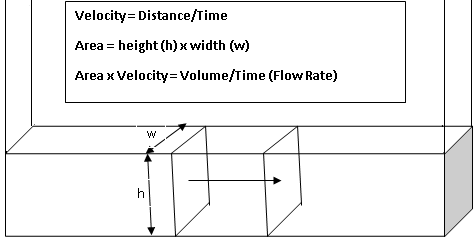
\includegraphics[scale=0.5]{ChannelFlow3}
\end{center}
$Flow (Q) = Velocity (V) * Area (A)$\\
$\implies Flow\Big[ 14 \dfrac{MG}{day}* \dfrac{10^6 gal}{MG} * \dfrac{ft^3}{7.48 gal}*\dfrac{day}{24*60*60sec}\Big]\dfrac{ft^3}{sec} = Velocity(V) \dfrac{ft}{sec}* Area (6 * 2) ft ^2$\\
\vspace{0.2cm}
$\implies 21.7 \dfrac{ft^3}{sec}= V\dfrac{ft}{sec}*12ft^2$\\
$\implies V \dfrac{ft}{sec}= \dfrac{21.7\dfrac{\cancelto{ft}{ft^3}}{sec}}{12\cancelto{}{ft^2}}= \boxed{1.8\dfrac{ft}{sec}}$\\

\item If a chemical is added in a sewer where wastewater is flowing at a velocity of 3.1 feet per second, how many minutes would it take for the chemical to reach the plant 7 miles away?\\
Solution:\\
Min $= \dfrac{1}{3.1}\dfrac{sec}{ft}*\dfrac{5280ft}{mile}*7 miles*\dfrac{min}{60 sec} = \boxed{199 min}$
\\

\item A plastic float takes 9.8 seconds to travel a distance of 25 feet in a wastewater channel. The channel is 3 ft 8 in. wide and the water level in this channel is 28 inches. What is the wastewater flow in GPM\\
Solution:\\
\vspace{0.3cm}
$Q=V*A$\\
$\implies Q=\dfrac{25ft}{9.8s}*\Big((3+\dfrac{8}{12})*\dfrac{28}{12}\Big)ft^2*7.48\dfrac{gal}{ft^3}*60\dfrac{s}{min}=\boxed{9,795\dfrac{gal}{min}}$



\item Calculate the flow, in gpd, that would pass through a grit chamber 2 feet wide, at a depth of 6 inches, with a velocity of 1 ft /sec\\
Solution:\\
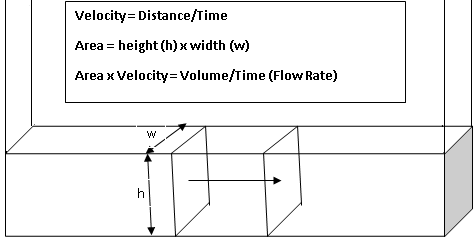
\includegraphics[scale=0.5]{ChannelFlow3}\\
$Q=V*A$\\
$Q=1\dfrac{ft}{s}*(2*0.5)ft^2=1\dfrac{ft^3}{s}$\\
$Q=1\dfrac{\cancel{ft^3}}{\cancel{s}}*\dfrac{(1440*60)\cancel{s}}{day}*7.48\dfrac{gal}{\cancel{ft^3}}=\boxed{646,272\dfrac{gal}{day}}$
\end{enumerate}



\subsection{Practice Problems} \index{Practice Problems}

\begin{enumerate}
\item A wastewater channel is 3.25 feet wide and is conveying a wastewater flow of 3.5 MGD. The wastewater flow is 8 inches deep. Calculate the velocity of this flow.\\

\item A plastic float is dropped into a wastewater channel and is found to travel 10 feet in 4.2 seconds. The channel is 2.4 feet wide and is flowing 1.8 feet deep. Calculate the flow rate of this wastewater in cubic feet per second.\\

\item A 12 inch pipe conveys sewage at 2.6 feet per second.  What is the flow expressed in MGD?

\item A sewer line to a wastewater treatment plant is 12 miles long. If the wastewater is flowing at 2.2 fps, approximately.  How long will it take for wastewater to reach the plant?\\
 
\end{enumerate}
\newpage

\section{Preliminary Treatment}\index{Preliminary Treatment}

\subsection{Example Problems} \index{Example Problems}

\begin{enumerate}

\item At a wastewater treatment plant which receives a flow rate of 650,000 gallons per day, a total of 50 cubic feet of grit was removed for the month. Calculate the rate of grit removal assuming 30 days in a month.\\
Solution:\\
$Grit Removal\dfrac{ft^3}{MG}=50\dfrac{ft^3}{ \cancel{month}}*\dfrac{\cancel{month}}{30\cancel{days}}*\dfrac{\cancel{day}}{650,000\cancel{gal}}*1,000,000\dfrac{\cancel{gal}}{MG}=\boxed{2.6\dfrac{ft^3}{MG}}$

\end{enumerate}

\subsection{Practice Problems} \index{Practice Problems}

\begin{enumerate}
\item On an average a 12.5 yd. load of grit is hauled to the landfill once every 20 days. Plant flow averages 12.5 MGD. Calculate the rate of grit collection in ft$^3$/MG.\\

\item On an average, 2 inches of grit is collected and removed every day in a 2.2 feet wide, 205 feet long grit channel.  Knowing the average flow through that grit channel is 10 MGD calculate the rate of grit collection in ft$^3$/MG\\

\end{enumerate}

\newpage
\section{Primary Treatment} \index{Primary Treatment}
\subsection{Example Problems} \index{Example Problems}
\begin{enumerate}
\item If a clarifier has a capacity of 0.25 MG, what is the detention time in hours if it receives a flow of 3 MGD\\
Solution:\\
$Clarifier \enspace detention \enspace time \enspace (hr) = 	\dfrac{ Clarifier \enspace volume (MG)}{Influent \enspace flow \enspace (MG/hr)}$\\
\vspace{0.5cm}
$Clarifier \enspace detention \enspace time \enspace (hr) = 	\dfrac{0.25\cancel{MG}}{\dfrac{3\cancel{MG}}{\cancel{day}}*\dfrac{\cancel{day}}{24hrs}}=\boxed{2hrs}$\\

\item If a 90 ft diameter primary clarifier operating at water depth of 20 ft is treating a 12MGD flow, calculate the surface loading rate (gal/(day-sq.ft).\\
Solution:\\
$Clarifier \enspace hydraulic \enspace loading \enspace 	\Big(\dfrac{gpd}{ft^2}\Big) =\dfrac{\dfrac{12\cancel{MG}}{{day}}*\dfrac{10^6gal}{\cancel{MG}}}{0.785*90^2 ft^2}=\boxed{1,887gpd/ft^2}$\\


\vspace{0.5cm}
\item What is the weir overflow rate (gpd/ft) when treating a 15 MGD flow in a 105 ft diameter primary sedimentation tank operating at water depth of 20 ft.\\
\vspace{0.5cm}
Solution:\\
\vspace{0.5cm}
$Clarifier \enspace detention \enspace time \enspace (hr) = 	\dfrac{(0.785*105^2*20)\cancel{ft^3}}{\dfrac{15\cancel{MG}}{\cancel{day}}*\dfrac{10^6\cancel{gal}}{\cancel{MG}}*\dfrac{\cancel{ft^3}}{7.48\cancel{gal}}*\dfrac{\cancel{day}}{24hrs}}=\boxed{2.1hrs}$\\
\end{enumerate}

\subsection{Practice Problems} \index{Practice Problems}

\begin{enumerate}


\item A circular clarifier receives a flow of 11 MGD.  If the clarifier is 90 ft. in diameter and is 12 ft. deep, what is: a) the hydraulic/surface loading rate, b) weir overflow rate, and c) clarifier detention time in hours?\\

\item At a 2.5 MGD wastewater treatment plant the primary clarifier has a detention time of 2 hours. How many gallons does this clarifier hold?\\

\end{enumerate}

\newpage

\section{Pumping}\index{Pumping}

\subsection{Example Problems} \index{Example Problems}


\begin{enumerate}

\item How many lbs/day of solids are removed in a clarifier treating a 6 MGD flow if the average inlet concentration is 320 mg/l and its average outlet concentration is 80 mg/l\\
\vspace{0.5cm}
Solution:\\
\vspace{0.5cm}
Applying pounds formula:\\
$\dfrac{lbs \enspace solids \enspace removed}{day}=6MGD*(320-80)\dfrac{mg}{l}*8.34=\boxed{120,096\dfrac{lbs \enspace solids}{day}}$

\item A clarifier has a TSS removal efficiency of 50\%.  If the influent TSS concentration is 220 mg/L, how many lbs/day of TSS are removed if the flow is 10 MGD.  Also, how many cu. ft of sludge is pumped if the sludge has a TS concentration of 5\%.\\
$lbs \enspace solids \enspace removed=(220*0.50)mg/l*10MGD*8.34=9,174lbs \enspace solids \enspace per \enspace day$
$$\dfrac{ft^3\enspace sludge}{day}= \dfrac{9,174 \enspace \cancel{lbs \enspace solids}}{day} * \dfrac{1 \enspace \cancel{lb \enspace sludge}}{0.05\enspace \cancel{lbs \enspace solids}}*\dfrac{\cancel{gal \enspace sludge}}{8.34\cancel{lb \enspace sludge}}*\dfrac{ft^3 \enspace sludge}{7.48 \enspace \cancel{gal}}=\boxed{2,941\dfrac{ft^3 \enspace sludge}{day}} $$

\item Given the tank is 10ft wide, 12 ft long and 18 ft deep tank including 2 ft of freeboard when filled to capacity. How much time (minutes) will be required to pump down this tank to a depth of 2 ft when the tank is at maximum capacity using a 600 GPM pump\\
Solution:\\
\vspace{0.5cm}

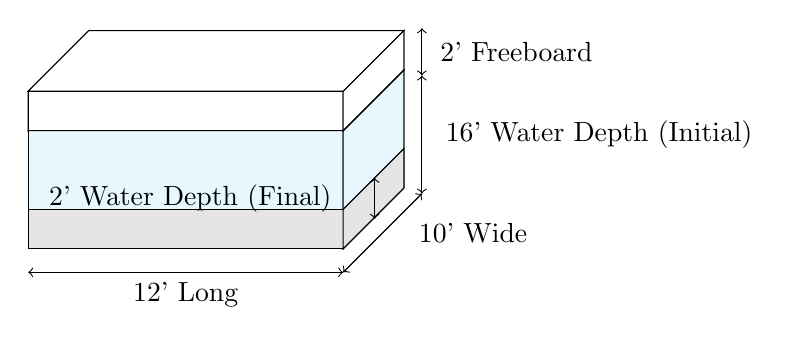
\begin{tikzpicture}

\pgfmathsetmacro{\cubexx}{4}
\pgfmathsetmacro{\cubeyy}{1.5}
\pgfmathsetmacro{\cubezz}{2}
\pgfmathsetmacro{\cubex}{4}
\pgfmathsetmacro{\cubey}{0.5}
\pgfmathsetmacro{\cubez}{2}
\pgfmathsetmacro{\cubexxx}{4}
\pgfmathsetmacro{\cubeyyy}{4}
\filldraw [fill=cyan!10!white, draw=black] (0,-\cubey,0) -- ++(-\cubexx,0,0) -- ++(0,-\cubeyy,0) -- ++(\cubexx,0,0) -- cycle ;
\filldraw [fill=cyan!0!white, draw=black] (0,-\cubey,0) -- ++(0,0,-\cubezz) -- ++(0,-\cubeyy,0) -- ++(0,0,\cubezz) -- cycle;
\filldraw [fill=cyan!10!white, draw=black] (0,-\cubey,0) -- ++(0,0,-\cubezz) -- ++(0,-\cubeyy,0) -- ++(0,0,\cubezz) -- cycle;
%\filldraw [fill=cyan!10!white, draw=black] (0,-\cubey,0) -- ++(-\cubexx,0,0) -- ++(0,0,-\cubezz) -- ++(\cubexx,0,0) -- cycle;
%%%\draw (0,-0.5,0) -- ++(-\cubex,0,0) -- ++(0,-\cubey,-\cubez) -- ++(\cubex,0,0) -- cycle;
\draw (-\cubex,0,0) -- ++(0,0,-\cubez) -- ++(0,-\cubey,0) -- ++(0,0,\cubez) -- cycle;
\draw (0,-\cubey,0) -- ++(-\cubex,0,0) -- ++(0,0,-\cubez) -- ++(\cubex,0,0) -- cycle;
\filldraw [fill=white, draw=black] (0,0,0) -- ++(-\cubex,0,0) -- ++(0,-\cubey,0) -- ++(\cubex,0,0) -- cycle ;
\filldraw [fill=white, draw=black] (0,0,0) -- ++(0,0,-\cubez) -- ++(0,-\cubey,0) -- ++(0,0,\cubez) -- cycle;
\filldraw [fill=white, draw=black] (0,0,0) -- ++(0,0,-\cubez) -- ++(0,-\cubey,0) -- ++(0,0,\cubez) -- cycle;
\filldraw [fill=white, draw=black] (0,0,0) -- ++(-\cubex,0,0) -- ++(0,0,-\cubez) -- ++(\cubex,0,0) -- cycle;

\filldraw [fill=Black!10!white, draw=black] (0,-1.5,0) -- ++(-\cubex,0,0) -- ++(0,-\cubey,0) -- ++(\cubex,0,0) -- cycle ;

\filldraw [fill=Black!10!white, draw=black] (0,-1.5,0) -- ++(0,0,-\cubez) -- ++(0,-\cubey,0) -- ++(0,0,\cubez) -- cycle;



%%\draw (0,-0.5,0) -- ++(-\cubex,0,0) -- ++(0,0,-\cubez) -- ++(\cubex,0,0) -- cycle;
%%\filldraw [fill=white, draw=black] (-\cubex,0,0) -- ++(0,0,-\cubez) -- ++(0,-\cubey,0) -- ++(0,0,\cubez) -- cycle;
%%\filldraw [fill=white, draw=black] (0,-\cubey,0) -- ++(-\cubex,0,0) -- ++(0,0,-\cubez) -- ++(\cubex,0,0) -- cycle ;

\draw [<->] (-4,-2.3) -- (0,-2.3) node [midway, below] {12' Long};
\draw [<->] (1,-1.3) -- (1,.2) node [midway, midway] {\hspace{4.5cm}16' Water Depth (Initial)};
\draw [<->] (0.4,-1.62) -- (0.4,-1.1) node [midway, midway] {\hspace{-4.8cm} 2' Water Depth (Final)};
\draw [<->] (1,.8) -- (1,.2) node [midway, midway] {\hspace{2.4cm}2' Freeboard};
\draw [<->] (1,-1.3) -- (0,-2.3) node [midway, midway] {\hspace{2.3cm}10' Wide};
\end{tikzpicture}\\
Volume to be pumped=$12 \enspace ft*10 \enspace ft *(16-2)\enspace ft=1,680ft^3$\\
\vspace{0.3cm}
$\implies \dfrac{1,680\cancel{ft^3}*7.48\dfrac{\cancel{gal}}{\cancel{ft^3}}}{600\dfrac{\cancel{gal}}{min}}=\boxed{21min}$

\end{enumerate}

\subsection{Practice Problems} \index{Practice Problems}

\begin{enumerate}
\item A sludge pump is set to pump 5 minutes each hour. It pumps at the rate of 35 gpm. How many gallons of sludge are pumped each day?\\

\item A community has a total flow of 15 MGD which is passed through a primary treatment plant which removes 60\% of the TSS and 35\% of the BOD. The average strength of the influent is 400 mg/l TSS and 275 mg/l BOD. If the total solids of the raw sludge is 5\%, how many cu. ft of sludge is pumped daily?\\

\item How many lbs of solids are removed daily by a primary clarifier treating a 6 MGD flow if the average influent TSS concentration is 300 mg/l and the clarifier TSS removal efficiency is 67\%?\\

\end{enumerate}

